\documentclass[../main.tex]{subfiles}

\begin{document}

    \begin{itemize}
        \item \textbf{Kaskadowe arkusze stylów} (ang. Cascading Style Sheets) - język opisu sposoby prezentacji (wyglądu) dokumentu HTML.
        \item CSS umożliwia \textbf{rozdzielenie struktury} i zawartości dokumentu od \textbf{sposobu} jego \textbf{prezentacji}.\\

        \item Określanie \textbf{czcionek}, \textbf{marginesów}, \textbf{odstępów} między liniami; \textbf{rozmiarów} i \textbf{położenia} poszczególnych elementów
        strony; \textbf{obramowań} i \textbf{wypełnień}.
        \item Zmiana sposobu \textbf{prezentacji standardowych elementów} (np. punktory w listach).
    \end{itemize}

    \subsection{Selektory}
    \begin{itemize}
        \item Selektor decyduje do \textbf{którego elementu} strony są stosowane właściwości.
        \item Kryterium wyboru może być m.in. typ elementu, atrybuty (w szczególności id i class) oraz położenie elementu względem innych elementów.
        \item Pseudo-elementy dają dostęp m.in. do fragmentów elementów (::first-letter).
        \item Można także używać pseudo-klas dających dostęp do informacji nie zawartych bezpośrednio w dokumencie (:hover, :visited).
    \end{itemize}

    \begin{table}[H]
        \begin{center}
            \begin{tabular}{|p{3.5cm}||p{4.5cm}|p{8cm}|}
                \hline
                \textbf{Selector} & \textbf{Example} & \textbf{Example description}\\
                \hline
                \hline
                \textbf{.class} & .intro & Selects all elements with class="intro"\\
                \hline
                \textbf{\#id} & \#firstname & Selects the element with id="firstname"\\
                \hline
                \textbf{*} & * & Selects all elements\\
                \hline
                \textbf{element} & p & Selects all <p> elements\\
                \hline
                \textbf{element,element} & div, p & Selects all <div> elements and all <p> elements\\
                \hline
                \textbf{element element} & div p & Selects all <p> elements inside <div> elements\\
                \hline
                \textbf{[attribute]} & [target] & Selects all elements with a target attribute\\
                \hline
                \textbf{[attribute=value]} & [target=\_blank] & Selects all elements with target="\_blank"\\
                \hline
            \end{tabular}
        \end{center}
    \end{table}

    \subsection{Priorytety}
    \begin{table}[H]
        \begin{center}
            \begin{tabular}{|p{1.5cm}|p{4cm}|p{10.5cm}|}
                \hline
                \textbf{Priority} & \textbf{CSS source type} & \textbf{Description}\\
                \hline
                \hline
                1 & Importance & The !important annotation overwrites the previous priority types\\
                \hline
                2 & Inline & A style applied to an HTML element via HTML 'style' attribute\\
                \hline
                3 & Media Type & A property definition applies to all media types, unless a media specific CSS is defined\\
                \hline
                4 & User defined & Most browsers have the accessibility feature: a user defined CSS\\
                \hline
                5 & Selector specificity & A specific contextual selector overwrites generic definition\\
                \hline
                6 & Rule order & Last rule declaration has a higher priority\\
                \hline
                7 & Parent inheritance & If a property is not specified, it is inherited from a parent element\\
                \hline
                8 & CSS property definition in HTML document & CSS rule or CSS inline style overwrites a default browser value\\
                \hline
                9 & Browser default & The lowest priority: browser default value is determined by W3C initial value specifications\\
                \hline
            \end{tabular}
        \end{center}
    \end{table}
    Style związane z fontami są dziedziczone z elementu rodzica. Większość pozostałych stylów nie jest dziedziczona.

    \subsection{Specyficzność}
    Specyficzność określa "\textbf{szczegółowość}" selektora:
    \begin{table}[H]
        \begin{center}
            \begin{tabular}{p{3cm} p{9cm} p{3cm}}
                0, 0 , 0, \textbf{1} & prosty selektor (selektor \textbf{elementu}) & (p)\\
                0, 0 , \textbf{1}, 0 & selektor \textbf{klasy} & (.head-button)\\
                0, \textbf{1} , 0, 0 & selektor oparty na \textbf{id} & (\#save-button)\\
                \textbf{1}, 0 , 0, 0 & style \textbf{inline} &\\
            \end{tabular}
        \end{center}
    \end{table}
    Selector "body \#content .data img:hover" ma specyficzność równą 0,1,2,2.

    \subsection{Box Model}
    \begin{table}[H]
        \begin{center}
            \begin{tabular}{p{8cm} p{8cm}}
                \begin{itemize}
                    \item Każdy element HTML można traktować jako \textbf{prostokąt}.
                    \item Zawartość elementu (\textbf{content}) jest otoczona wypełnieniem (\textbf{padding}), obramowaniem (\textbf{border}) oraz marginesem (\textbf{margin}).
                    \item W zależności od wartości box-sizing (\textbf{content-box} lub \textbf{border-box}) obliczany jest całkowity rozmiar elementu.
                \end{itemize}
                &
                \raisebox{-\totalheight}{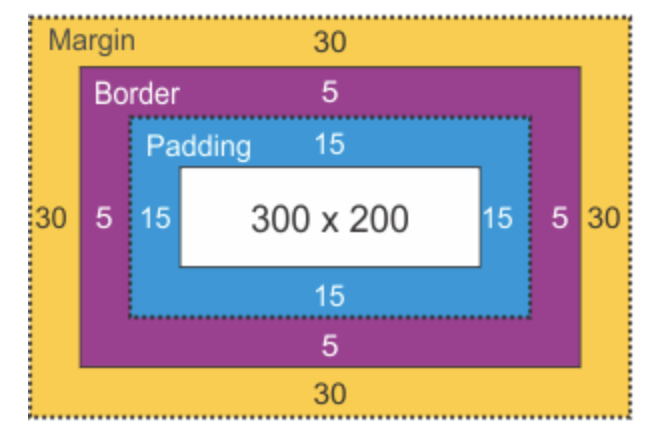
\includegraphics[width=8cm]{boxmodel.png}}
                \\
            \end{tabular}
        \end{center}
    \end{table}

    \subsection{Dodatki}
    \begin{itemize}
        \item \textbf{CSS Transforms} - pozwala na transformacje takie jak przesunięcie, skalowanie, obracanie, itp.
        \item \textbf{CSS Transitions} - pozwala na płynną zmianę wartości.
        \item \textbf{SS Flexbox Layout}
        \begin{itemize}
            \item Elastyczny \textbf{menadżer układu elementów} na stronie.
            \item Elementy mogą być typu flex-container i/lub flex-item.
            \item Dla \textbf{flex-container} możemy określić \textbf{kierunek i sposób ułożenia} elementów flex-item (pionowo/poziomo, prawo/lewo, zawijanie wierszy, wykorzystanie wolnej przestrzeni).
            \item Dla \textbf{flex-item} możemy okreslić \textbf{zdolnośc elementu} do powiększania/zmniejszania, wypełniania pustej przestrzeni, bazowy rozmiar, kolejność wyświetlania, itp.
            \item Stosunkowo łatwo wykonac \textbf{podział strony} na kilka \textbf{kolumn} tej samej wysokości.
        \end{itemize}
    \end{itemize}
\end{document}